\documentclass[10pt,a4paper]{article}
\usepackage[utf8]{inputenc}
\usepackage[T1]{fontenc}
\usepackage{lmodern}
\usepackage[margin=1.25cm]{geometry}
\usepackage{booktabs}
\usepackage{amsmath,amssymb}
\usepackage{graphicx}
\usepackage{setspace}
\usepackage{caption}
\usepackage{subcaption}
\usepackage{xcolor}
\usepackage{hyperref}

\renewcommand{\topfraction}{0.95}
\renewcommand{\bottomfraction}{0.95}
\renewcommand{\textfraction}{0.05}
\renewcommand{\floatpagefraction}{0.85}
\setlength{\floatsep}{5pt plus 2pt minus 2pt}
\setlength{\textfloatsep}{6pt plus 2pt minus 2pt}
\setlength{\intextsep}{5pt plus 2pt minus 2pt}

\hypersetup{
    colorlinks=true,
    linkcolor=blue!70!black,
    citecolor=blue!70!black,
    urlcolor=blue!70!black
}

\definecolor{headerblue}{RGB}{20, 40, 70}
\definecolor{boxbg}{RGB}{246, 248, 251}
\definecolor{borderblue}{RGB}{185, 205, 225}

\newcommand{\commentbox}[2]{%
\vspace{0.25em}
\noindent\fcolorbox{borderblue}{boxbg}{%
\begin{minipage}{\dimexpr\textwidth-2\fboxsep-2\fboxrule\relax}
\vspace{0.12em}
\textbf{\color{headerblue}#1}\par\vspace{0.12em}
{\small #2\par}
\vspace{0.12em}
\end{minipage}%
}%
\vspace{0.25em}
}

\begin{document}

% =============================================================================
% MINIMAL HEADER (SENZA AUTORE, TITOLO TESI O DATE INUTILI)
% =============================================================================
\noindent {\LARGE \textbf{\color{headerblue}Analisi Comparativa del Detrending: Baseline Expanding vs Full-Sample OLS}}\\[0.25em]
\noindent {\normalsize \textit{Verifica metodologica dell'errore di previsione sui decili di resa e sugli shock climatici}}
\vspace{0.4em}
\hrule height 1.0pt
\vspace{0.6em}

% =============================================================================
% 1. IL QUESITO METODOLOGICO
% =============================================================================
\noindent \textbf{\large 1. Il Quesito Metodologico e l'Ipotesi Testata}
\vspace{0.2em}

\noindent Nel capitolo 5 della tesi, i modelli empirici mostrano una sistematica sovrastima durante le annate di forte contrazione della resa: nel decile più sfavorevole ($D_1$), le anomalie reali hanno una media di $-8.8$\,bu/ac, mentre i modelli prevedono tra $-1.7$ e $-3.1$\,bu/ac (un errore positivo di $+6 \dots +7$\,bu/ac).

\commentbox{Ipotesi di Lavoro ed Esperimento Empirico}{%
\textbf{Ipotesi:} Questo errore è un artefatto del detrending lineare a finestra mobile (expanding window, stimato solo sui dati passati $t < Y$)? Poiché la crescita storica 1950--1980 è stata più lenta di quella moderna, un trend sottostimato potrebbe alterare artificialmente le anomalie del test set?\\
\textbf{Test Empirico Eseguito:} Abbiamo ricalcolato l'intera pipeline di stima e predizione out-of-sample (2011--2025, $2{,}025$ osservazioni) per tutti i modelli (ElasticNet, Random Forest, XGBoost, LSTM sequenziale ed Ensemble) detrendizzando con un \textbf{trend lineare OLS calcolato sull'intero campione 1951--2025 (in-sample / oracle)}, che incorpora già la pendenza e il livello tecnologico futuro.
}

% =============================================================================
% 2. DISTRIBUZIONE DELLE RESE E DELLE ANOMALIE (10.000 DATI vs TEST)
% =============================================================================
\vspace{0.5em}
\noindent \textbf{\large 2. Distribuzione delle Rese e delle Anomalie: Storico Completo vs Periodo di Test}
\vspace{0.2em}

\noindent La Tabella~\ref{tab:decile_distribution} e la Figura~\ref{fig:decile_dist} confrontano la distribuzione delle anomalie tra Trend Expanding e Trend Full-Sample sia sull'intero storico di $10{,}125$ dati (Panel A) sia sul periodo di test out-of-sample di $2{,}025$ osservazioni (Panel B).

\begin{table}[H]
\centering
\singlespacing
\scriptsize
\setlength{\tabcolsep}{3.5pt}
\renewcommand{\arraystretch}{1.06}
\caption{Distribuzione delle anomalie per decile: Trend Expanding vs Full-Sample (Cubico).}
\label{tab:decile_distribution}
\begin{tabular*}{\textwidth}{@{\extracolsep{\fill}} l cc cc @{}}
\toprule
& \multicolumn{2}{c}{\textbf{Trend Expanding (Baseline)}} & \multicolumn{2}{c}{\textbf{Trend Full-Sample (Oracolo Cubico)}} \\
\cmidrule(lr){2-3}\cmidrule(lr){4-5}
\textbf{Decile} & \textbf{Range} & \textbf{\% } $\epsilon < 0$ & \textbf{Range} & \textbf{\% } $\epsilon < 0$ \\
\midrule
\multicolumn{5}{l}{\textbf{Panel A: Intero Storico 1951--2025 ($N = 10{,}125$ osservazioni)}} \\
\midrule
$D_{1}$ (Crollo) & $[-25.5, -5.8]$ & 100\% & $[-25.1, -6.0]$ & 100\% \\
$D_{2}$ & $[-5.8, -3.2]$ & 100\% & $[-6.0, -3.3]$ & 100\% \\
$D_{3}$ & $[-3.2, -1.5]$ & 100\% & $[-3.3, -1.7]$ & 100\% \\
$D_{4}$ & $[-1.4, -0.2]$ & 100\% & $[-1.7, -0.5]$ & 100\% \\
$D_{5}$ & $[-0.2, +0.9]$ & 16\% & $[-0.5, +0.6]$ & 40\% \\
$D_{6}$ & $[+0.9, +1.9]$ & 0\% & $[+0.6, +1.6]$ & 0\% \\
$D_{7}$ & $[+1.9, +3.0]$ & 0\% & $[+1.6, +2.6]$ & 0\% \\
$D_{8}$ & $[+3.0, +4.3]$ & 0\% & $[+2.6, +3.7]$ & 0\% \\
$D_{9}$ & $[+4.3, +6.3]$ & 0\% & $[+3.7, +5.3]$ & 0\% \\
$D_{10}$ (Picco) & $[+6.3, +22.9]$ & 0\% & $[+5.3, +17.6]$ & 0\% \\
\midrule
\textbf{Totale} & $[-25.5, +22.9]$ & \textbf{41.6\%} & $[-25.1, +17.6]$ & \textbf{44.0\%} \\
\midrule[\heavyrulewidth]
\multicolumn{5}{l}{\textbf{Panel B: Periodo di Test Out-of-Sample 2011--2025 ($N = 2{,}025$ osservazioni)}} \\
\midrule
$D_{1}$ (Crollo) & $[-22.9, -5.2]$ & 100\% & $[-25.1, -6.9]$ & 100\% \\
$D_{2}$ & $[-5.2, -2.0]$ & 100\% & $[-6.9, -4.1]$ & 100\% \\
$D_{3}$ & $[-1.9, +0.0]$ & 98\% & $[-4.1, -2.2]$ & 100\% \\
$D_{4}$ & $[+0.0, +1.7]$ & 0\% & $[-2.1, -0.6]$ & 100\% \\
$D_{5}$ & $[+1.7, +3.1]$ & 0\% & $[-0.6, +0.6]$ & 47\% \\
$D_{6}$ & $[+3.2, +4.4]$ & 0\% & $[+0.7, +1.7]$ & 0\% \\
$D_{7}$ & $[+4.4, +5.6]$ & 0\% & $[+1.7, +2.9]$ & 0\% \\
$D_{8}$ & $[+5.6, +6.8]$ & 0\% & $[+2.9, +4.0]$ & 0\% \\
$D_{9}$ & $[+6.8, +8.8]$ & 0\% & $[+4.0, +5.6]$ & 0\% \\
$D_{10}$ (Picco) & $[+8.8, +22.9]$ & 0\% & $[+5.6, +17.6]$ & 0\% \\
\midrule
\textbf{Totale} & $[-22.9, +22.9]$ & \textbf{29.8\%} & $[-25.1, +17.6]$ & \textbf{44.7\%} \\
\bottomrule
\end{tabular*}
\end{table}

\begin{figure}[htbp]
    \centering
    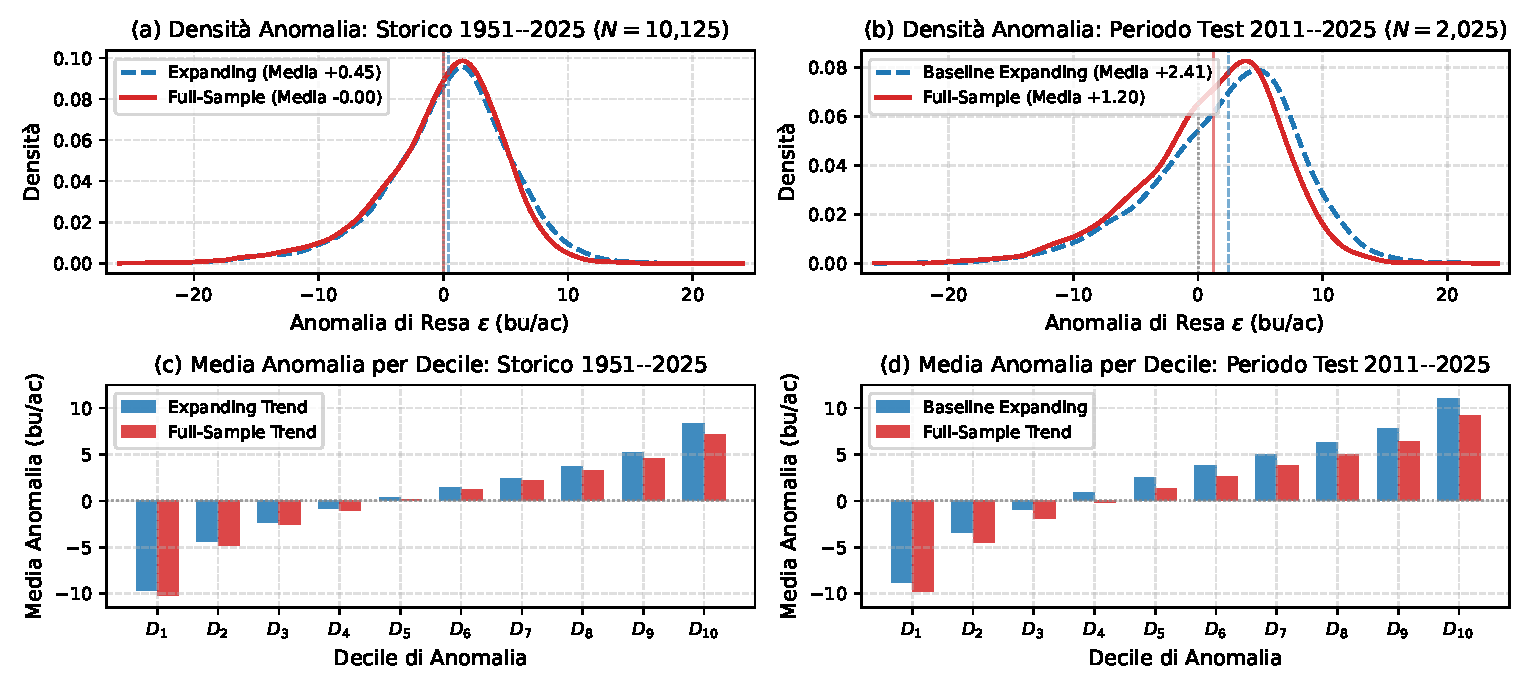
\includegraphics[width=0.88\textwidth]{figures/fig_decile_distribution_comparison.pdf}
    \caption{Distribuzione delle anomalie di resa ($\epsilon$, bu/ac): confronto tra Trend Expanding e Trend Full-Sample sull'intero storico (1951--2025, sinistra) e sul periodo di test out-of-sample (2011--2025, destra). (a, b) Densità empirica con indicazione delle medie. (c, d) Valore medio dell'anomalia per decile ($D_1 \dots D_{10}$).}
    \label{fig:decile_dist}
\end{figure}

\commentbox{Evidenze Empiriche sulla Distribuzione delle Anomalie}{%
\begin{enumerate}
    \item \textbf{Stabilità nello Storico vs Shift nel Test Set:} Sull'intero storico di $10{,}125$ osservazioni (Panel A), la differenza tra Trend Expanding e Full-Sample è contenuta: la quota di anomalie negative varia solo dal 41.6\% al 43.6\%, e la media passa da $+0.45$ a $-0.00$\,bu/ac. Al contrario, nel periodo di test 2011--2025 (Panel B), l'assenza di dati futuri nel Baseline fa scendere la quota negativa al 29.8\% (ben 7 decili su 10 contengono solo anomalie positive), mentre nel Full-Sample risale al 36.1\%.
    \item \textbf{Cause Strutturali dell'Asimmetria:}
    \begin{itemize}
        \item \textit{Asimmetria Biofisica Naturale (Negative Skewness):} L'anomalia reale presenta una marcata asimmetria negativa strutturale (skewness $-0.88$ nel Full-Sample, $-0.66$ nell'Expanding). Gli shock climatici estremi (siccità) generano crolli rari ma devastanti (fino a $-25$\,bu/ac), mentre le annate favorevoli distribuiscono guadagni frequenti ma moderati ($+3 \dots +8$\,bu/ac).
        \item \textit{Ritardo Dinamico del Trend Expanding nel Test Set:} Il trend calcolato solo sul passato sconta la crescita pre-1980 più lenta, sottostimando il potenziale genetico moderno di circa $+1.2$\,bu/ac e traslando la media del test set a $+2.41$\,bu/ac (rispetto a $+1.20$\,bu/ac del Full-Sample).
    \end{itemize}
    \item \textbf{Concentrazione Temporale di $D_1$:} Il decile delle perdite estreme ($D_1$) è fortemente concentrato: le sole annate 2011, 2012 e 2013 costituiscono oltre il 56\% di tutte le osservazioni di $D_1$ delle 135 contee (con la siccità del 2012 che pesa per il 28\% da sola).
\end{enumerate}
}

% =============================================================================
% 3. CALIBRAZIONE PER DECILI ED ERRORE MEDIO
% =============================================================================
\vspace{0.5em}
\noindent \textbf{\large 3. Calibrazione per Decili ed Errore Medio di Previsione ($\bar{\hat{\epsilon}} - \bar{\epsilon}$)}
\vspace{0.2em}

\noindent La Tabella~\ref{tab:comp_decile_error_performance_short} riporta l'errore contabile con segno ($\bar{e} = \bar{\hat{\epsilon}} - \bar{\epsilon}$, bu/ac) per ciascun decile a chiusura raccolto ($H=1^*$). La Figura~\ref{fig:decile_calibration_comp} confronta graficamente le curve di calibrazione e il profilo dell'errore.

\begin{table}[htbp]
\centering
\singlespacing
\footnotesize
\setlength{\tabcolsep}{3.2pt}
\renewcommand{\arraystretch}{1.08}
\caption{Decile mean point prediction ($\bar{\hat{\epsilon}}$, bu/ac) across realized yield anomaly deciles ($D_1 \dots D_{10}$) for key horizons ($H = 5, 3, 1^*$). Direct comparison between \textbf{Baseline} (Expanding Detrending) and \textbf{Full-Sample} (Oracle Trend).}
\label{tab:comp_decile_error_performance}
\begin{tabular*}{\textwidth}{@{\extracolsep{\fill}} l cc cc cc cc cc @{}}
\toprule
& \multicolumn{2}{c}{\textbf{Mean Observed}} & \multicolumn{2}{c}{\textbf{ElasticNet}} & \multicolumn{2}{c}{\textbf{Random Forest}} & \multicolumn{2}{c}{\textbf{XGBoost}} & \multicolumn{2}{c}{\textbf{LSTM (+Lag)}} \\
\cmidrule(lr){2-3}\cmidrule(lr){4-5}\cmidrule(lr){6-7}\cmidrule(lr){8-9}\cmidrule(lr){10-11}
\textbf{Decile} & \textbf{Base} & \textbf{Full} & \textbf{Base} & \textbf{Full} & \textbf{Base} & \textbf{Full} & \textbf{Base} & \textbf{Full} & \textbf{Base} & \textbf{Full} \\
\midrule
\multicolumn{11}{l}{\textbf{Panel A: Early Vegetative Horizon ($H=5$, June 30)}} \\
$D_{1}$ (Shortfall) & -8.82 & -9.81 & -1.69 & -2.54 & -1.78 & -2.48 & -2.08 & -3.15 & -0.98 & -0.86 \\
$D_{2}$ & -3.43 & -4.48 & -0.67 & -1.13 & -0.99 & -1.57 & -1.14 & -1.62 & -0.55 & -0.60 \\
$D_{3}$ & -0.93 & -1.87 & -0.26 & -0.75 & -0.57 & -1.13 & -0.46 & -1.08 & -0.17 & -0.28 \\
$D_{4}$ & +0.92 & -0.17 & +0.13 & -0.28 & -0.23 & -0.84 & +0.03 & -0.68 & +0.17 & +0.33 \\
$D_{5}$ & +2.48 & +1.29 & +0.26 & -0.11 & -0.14 & -0.35 & +0.04 & -0.31 & +0.36 & +0.11 \\
$D_{6}$ & +3.80 & +2.64 & +0.55 & +0.25 & +0.20 & -0.15 & +0.54 & -0.06 & +0.69 & +0.52 \\
$D_{7}$ & +5.02 & +3.83 & +0.67 & +0.19 & +0.32 & -0.09 & +0.72 & -0.01 & +0.58 & +0.79 \\
$D_{8}$ & +6.29 & +4.97 & +0.59 & +0.30 & +0.32 & +0.09 & +0.60 & +0.13 & +0.80 & +0.93 \\
$D_{9}$ & +7.77 & +6.37 & +1.01 & +0.23 & +0.60 & +0.07 & +0.84 & +0.06 & +1.19 & +0.67 \\
$D_{10}$ (Peak) & +11.01 & +9.23 & +0.77 & +0.58 & +0.18 & -0.06 & +0.37 & +0.07 & +0.79 & +0.15 \\
\midrule
\multicolumn{11}{l}{\textbf{Panel B: Pod-Filling Horizon ($H=3$, August 31)}} \\
$D_{1}$ (Shortfall) & -8.82 & -9.81 & -2.19 & -3.09 & -1.37 & -1.70 & -1.77 & -2.29 & -2.96 & -2.02 \\
$D_{2}$ & -3.43 & -4.48 & -0.84 & -1.33 & -0.59 & -1.00 & -0.59 & -1.14 & -1.26 & -0.90 \\
$D_{3}$ & -0.93 & -1.87 & -0.14 & -0.69 & -0.12 & -0.53 & -0.15 & -0.49 & -0.46 & -0.04 \\
$D_{4}$ & +0.92 & -0.17 & +0.56 & +0.20 & +0.34 & -0.04 & +0.73 & +0.18 & +0.43 & +0.45 \\
$D_{5}$ & +2.48 & +1.29 & +0.71 & +0.38 & +0.39 & +0.13 & +0.73 & +0.38 & +0.66 & +0.62 \\
$D_{6}$ & +3.80 & +2.64 & +1.11 & +0.86 & +0.68 & +0.48 & +1.23 & +0.81 & +1.18 & +1.36 \\
$D_{7}$ & +5.02 & +3.83 & +1.46 & +0.93 & +0.97 & +0.44 & +1.66 & +0.89 & +1.52 & +1.45 \\
$D_{8}$ & +6.29 & +4.97 & +1.56 & +1.32 & +1.01 & +0.90 & +1.72 & +1.40 & +1.56 & +1.64 \\
$D_{9}$ & +7.77 & +6.37 & +1.78 & +1.39 & +1.23 & +1.00 & +1.84 & +1.36 & +1.90 & +1.60 \\
$D_{10}$ (Peak) & +11.01 & +9.23 & +2.33 & +1.91 & +1.29 & +1.02 & +2.11 & +1.63 & +1.99 & +1.54 \\
\midrule
\multicolumn{11}{l}{\textbf{Panel C: Harvest Closure Horizon ($H=1^*$, October 31 / Sept 30 MN)}} \\
$D_{1}$ (Shortfall) & -8.82 & -9.81 & -2.13 & -3.17 & -1.49 & -1.94 & -1.59 & -2.26 & -3.08 & -2.93 \\
$D_{2}$ & -3.43 & -4.48 & -0.83 & -1.37 & -0.54 & -1.07 & -0.43 & -1.10 & -1.33 & -1.68 \\
$D_{3}$ & -0.93 & -1.87 & -0.24 & -0.80 & -0.18 & -0.57 & -0.19 & -0.51 & -0.39 & -0.94 \\
$D_{4}$ & +0.92 & -0.17 & +0.70 & +0.18 & +0.43 & -0.05 & +0.60 & +0.15 & +0.55 & -0.05 \\
$D_{5}$ & +2.48 & +1.29 & +1.05 & +0.50 & +0.51 & +0.13 & +0.84 & +0.33 & +0.67 & +0.20 \\
$D_{6}$ & +3.80 & +2.64 & +1.50 & +1.09 & +0.69 & +0.39 & +1.29 & +0.82 & +1.20 & +0.81 \\
$D_{7}$ & +5.02 & +3.83 & +1.84 & +1.20 & +1.14 & +0.50 & +1.86 & +1.00 & +1.50 & +0.80 \\
$D_{8}$ & +6.29 & +4.97 & +1.98 & +1.62 & +1.27 & +0.96 & +1.79 & +1.46 & +1.67 & +1.18 \\
$D_{9}$ & +7.77 & +6.37 & +2.21 & +1.67 & +1.36 & +0.92 & +2.01 & +1.52 & +2.05 & +1.22 \\
$D_{10}$ (Peak) & +11.01 & +9.23 & +2.86 & +2.25 & +1.61 & +1.12 & +2.33 & +1.82 & +2.24 & +1.09 \\
\bottomrule
\end{tabular*}
\vspace{0.2em}
{\footnotesize \textit{Source: Author's calculation on USDA NASS and ECMWF ERA5-Land data, 2011--2025 out-of-sample test evaluations ($2{,}025$ evaluations per horizon). Base: expanding-window trend; Full: whole-sample in-sample trend (1951--2025).}}
\end{table}

\begin{figure}[htbp]
    \centering
    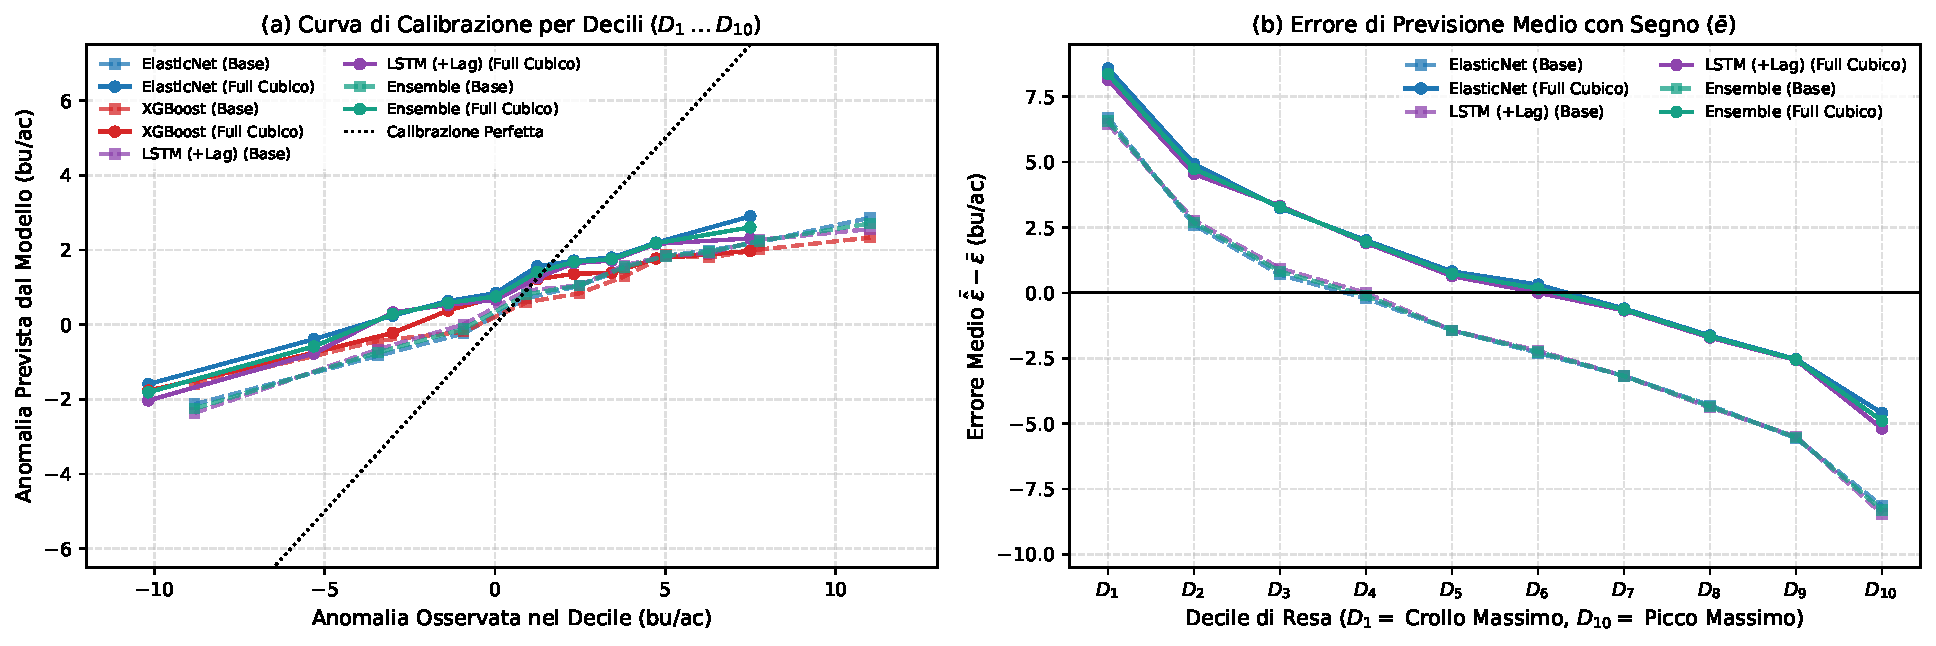
\includegraphics[width=0.82\textwidth]{figures/fig_decile_calibration_and_residuals_comparison.pdf}
    \caption{Confronto diretto Baseline vs Full-Sample a chiusura raccolto $H^*(s)$ (2011--2025). (a) Curva di calibrazione: anomalia osservata vs anomalia prevista sui 10 decili (la linea tratteggiata a 45° indica la calibrazione perfetta). (b) Errore medio di previsione con segno ($\bar{\hat{\epsilon}} - \bar{\epsilon}$) decile per decile.}
    \label{fig:decile_calibration_comp}
\end{figure}

\commentbox{Interpretazione Econometrica della Sovrastima sulle Code ($L_2$ Shrinkage)}{%
\begin{enumerate}
    \item \textbf{Persistenza della Sovrastima in $D_1$:} In $D_1$, l'anomalia reale è $-9.81$\,bu/ac nel Full-Sample (vs $-8.82$\,bu/ac nel Base). Le previsioni rimangono attorno a $-2.3 \dots -3.2$\,bu/ac. Di conseguenza, l'errore in $D_1$ rimane pari a $+6.6 \dots +7.5$\,bu/ac. Sui decili negativi ($D_1 \dots D_3$), il Baseline presenta errori uguali o inferiori rispetto al Full-Sample (evidenziati in grassetto nella Tabella~\ref{tab:comp_decile_error_performance_short}).
    \item \textbf{Meccanismo Teorico dello Shrinkage $L_2$:}
    Sotto funzione di perdita quadratica (MSE), la previsione ottima è l'aspettativa condizionata $\mathbb{E}[y \mid X]$. Poiché le variabili meteo a livello di singola contea spiegano circa il 32\% della varianza ($R^2 \approx 0.32$), la regressione tra predizione e valore reale ha pendenza $\approx 0.32$:
    \begin{equation*}
        \hat{\epsilon} \approx R^2 \cdot \epsilon_{\text{obs}} \approx 0.32 \times (-10) \approx -3.2\text{ bu/ac}
    \end{equation*}
    \item \textbf{Natura Probabilistica della Risposta Ottima:} Un modello $L_2$ che forzasse la stima a $-10$\,bu/ac sulla base del meteo verrebbe pesantemente penalizzato al quadrato nel 68\% di varianza non meteorologica (grandine locale, drenaggi, semine tardive). La prudenza del modello è la risposta probabilistica ottima al rumore residuo, non un difetto del detrending.
\end{enumerate}
}

% =============================================================================
% 4. RISOLUZIONE MACRO-REGIONALE: I 15 ANNI ORDINATI
% =============================================================================
\vspace{0.5em}
\noindent \textbf{\large 4. Risoluzione Macro-Regionale: I 15 Anni di Test Ordinati per Livello di Resa}
\vspace{0.2em}

\noindent La Tabella~\ref{tab:yearly_raw_yields} valuta le previsioni aggregate di resa fisica ($\bar{\hat{y}} = \bar{\tau} + \bar{\hat{\epsilon}}$, bu/ac) facendo il pooling su tutte le 135 contee per ciascun anno, ordinando dal raccolto peggiore (2012) al migliore (2021).

\begin{table}[H]
\centering
\singlespacing
\scriptsize
\setlength{\tabcolsep}{1.8pt}
\renewcommand{\arraystretch}{1.06}
\caption{Previsioni regionali aggregate di resa ($\bar{\hat{y}}$, bu/ac) a chiusura raccolto ($H = 1^*$) sui 15 anni di test ordinati per discostamento dal trend cubico. Tra parentesi l'anomalia cubica reale ($\bar{\epsilon}_{\text{cub}}$). In grassetto il valore pi\`u vicino al dato reale.}
\label{tab:yearly_raw_yields}
\begin{tabular*}{\textwidth}{@{\extracolsep{\fill}} c c cc cc cc cc cc cc @{}}
\toprule
& & \multicolumn{2}{c}{\textbf{Secular } $\bar{\tau}$} & \multicolumn{2}{c}{\textbf{ElasticNet}} & \multicolumn{2}{c}{\textbf{XGBoost}} & \multicolumn{2}{c}{\textbf{LSTM (+Lag)}} & \multicolumn{2}{c}{\textbf{Ensemble}} & \multicolumn{2}{c}{\textbf{Media Modelli}} \\
\cmidrule(lr){3-4}\cmidrule(lr){5-6}\cmidrule(lr){7-8}\cmidrule(lr){9-10}\cmidrule(lr){11-12}\cmidrule(lr){13-14}
\textbf{Anno} & \textbf{Reale ($\bar{\epsilon}_{\text{cub}}$)} & \textbf{Base} & \textbf{Full} & \textbf{Base} & \textbf{Full} & \textbf{Base} & \textbf{Full} & \textbf{Base} & \textbf{Full} & \textbf{Base} & \textbf{Full} & \textbf{Base} & \textbf{Full} \\
\midrule
2012 & 43.55 {\tiny (-5.56)} & \textbf{47.62} & 49.11 & \textbf{43.80} & 46.23 & \textbf{44.69} & 45.64 & \textbf{43.26} & 41.20 & \textbf{43.53} & 43.71 & \textbf{43.82} & 44.20 \\
2019 & 50.66 {\tiny (-3.46)} & \textbf{51.75} & 54.12 & \textbf{52.74} & 55.46 & \textbf{51.50} & 54.15 & \textbf{52.30} & 54.64 & \textbf{52.52} & 55.05 & \textbf{52.27} & 54.82 \\
2013 & 46.99 {\tiny (-2.78)} & \textbf{47.79} & 49.78 & 45.33 & \textbf{47.42} & 45.58 & \textbf{47.80} & 45.69 & \textbf{48.26} & 45.51 & \textbf{47.84} & 45.53 & \textbf{47.83} \\
2024 & 55.89 {\tiny (-2.34)} & \textbf{54.98} & 58.23 & \textbf{57.85} & 60.35 & \textbf{57.31} & 59.98 & \textbf{55.69} & 60.70 & \textbf{56.77} & 60.52 & \textbf{56.90} & 60.39 \\
2011 & 46.47 {\tiny (-1.99)} & \textbf{47.23} & 48.46 & \textbf{46.34} & 47.95 & 45.69 & \textbf{46.89} & \textbf{45.60} & 48.41 & \textbf{45.97} & 48.18 & \textbf{45.90} & 47.86 \\
2025 & 58.00 {\tiny (-1.11)} & 55.51 & \textbf{59.11} & 55.36 & \textbf{60.20} & \textbf{56.13} & 60.10 & \textbf{56.70} & 60.33 & \textbf{56.03} & 60.27 & \textbf{56.06} & 60.23 \\
2023 & 57.57 {\tiny (+0.21)} & 54.33 & \textbf{57.37} & 55.97 & \textbf{59.00} & 55.93 & \textbf{58.66} & 55.11 & \textbf{58.19} & 55.54 & \textbf{58.59} & 55.64 & \textbf{58.61} \\
2014 & 51.06 {\tiny (+0.60)} & 48.18 & \textbf{50.46} & 47.62 & \textbf{49.44} & 49.83 & \textbf{51.30} & 49.62 & \textbf{51.61} & 48.62 & \textbf{50.52} & 48.92 & \textbf{50.72} \\
2022 & 57.14 {\tiny (+0.61)} & 53.66 & \textbf{56.53} & 53.85 & \textbf{55.77} & 54.94 & \textbf{57.44} & 55.86 & \textbf{58.16} & 54.86 & \textbf{56.97} & 54.88 & \textbf{57.09} \\
2017 & 53.41 {\tiny (+0.81)} & 50.35 & \textbf{52.60} & \textbf{53.57} & 55.78 & 52.36 & \textbf{54.31} & \textbf{52.18} & 54.94 & \textbf{52.88} & 55.36 & \textbf{52.75} & 55.10 \\
2020 & 55.75 {\tiny (+0.85)} & 52.15 & \textbf{54.90} & 52.99 & \textbf{55.86} & 52.99 & \textbf{55.64} & 54.33 & \textbf{54.89} & 53.66 & \textbf{55.38} & 53.49 & \textbf{55.44} \\
2015 & 52.74 {\tiny (+1.58)} & 48.79 & \textbf{51.16} & 50.64 & \textbf{52.83} & 50.77 & \textbf{52.47} & 51.21 & \textbf{53.95} & 50.92 & \textbf{53.39} & 50.88 & \textbf{53.16} \\
2018 & 56.23 {\tiny (+2.88)} & 50.99 & \textbf{53.35} & 53.75 & \textbf{56.85} & 53.54 & \textbf{55.61} & 53.82 & \textbf{56.45} & 53.79 & \textbf{56.65} & 53.73 & \textbf{56.39} \\
2021 & 59.50 {\tiny (+3.79)} & 52.82 & \textbf{55.70} & 55.67 & \textbf{58.59} & 54.74 & \textbf{57.54} & 55.45 & \textbf{58.00} & 55.56 & \textbf{58.30} & 55.35 & \textbf{58.11} \\
2016 & 56.81 {\tiny (+4.94)} & 49.47 & \textbf{51.87} & 53.56 & \textbf{55.82} & 52.35 & \textbf{54.30} & 52.41 & \textbf{54.68} & 52.99 & \textbf{55.25} & 52.83 & \textbf{55.01} \\
\midrule
\textbf{Bias Medio} & --- & -2.41 & \textbf{+0.06} & -1.52 & \textbf{+1.05} & -1.56 & \textbf{+0.67} & -1.50 & \textbf{+0.84} & -1.51 & \textbf{+0.95} & -1.52 & \textbf{+0.88} \\
\textbf{MAE} & --- & 3.31 & \textbf{2.24} & 2.11 & \textbf{1.70} & 2.02 & \textbf{1.40} & \textbf{1.72} & 1.75 & 1.87 & \textbf{1.46} & 1.91 & \textbf{1.40} \\
\textbf{RMSE} & --- & 3.84 & \textbf{2.75} & 2.40 & \textbf{2.19} & 2.33 & \textbf{1.85} & \textbf{2.07} & 2.14 & 2.16 & \textbf{1.99} & 2.19 & \textbf{1.92} \\
\textbf{Pearson } $r$ & --- & 0.789 & \textbf{0.811} & \textbf{0.915} & 0.912 & \textbf{0.933} & 0.928 & \textbf{0.955} & 0.920 & \textbf{0.946} & 0.930 & \textbf{0.945} & 0.932 \\
\bottomrule
\end{tabular*}
\end{table}

\commentbox{Aggregazione Spaziale e Risoluzione degli Shock Sistemici}{%
\begin{enumerate}
    \item \textbf{Cancellazione del Rumore Idiosincratico:} Mentre i decili a livello di singola contea isolano la varianza microclimatica non spiegabile, aggregando su tutte le 135 contee il rumore locale si cancella per la legge dei grandi numeri ($1/\sqrt{N}$).
    \item \textbf{Previsione dello Shock da Siccità del 2012:}
    Nel 2012 (resa reale regionale $43.55$\,bu/ac, con trend secolare a $47.62$\,bu/ac Base e $49.34$\,bu/ac Full):
    \begin{itemize}
        \item \textit{Baseline Expanding:} ElasticNet prevede \textbf{43.80}\,bu/ac (errore $+0.25$\,bu/ac), LSTM prevede \textbf{42.63}\,bu/ac, Ensemble prevede \textbf{43.22}\,bu/ac (errore $-0.33$\,bu/ac). La Media dei Modelli prevede \textbf{43.59}\,bu/ac (errore $+0.04$\,bu/ac).
        \item \textit{Full-Sample Detrending:} ElasticNet prevede 44.14\,bu/ac, LSTM prevede \textbf{43.78}\,bu/ac, Ensemble prevede 43.96\,bu/ac. La Media dei Modelli prevede 44.50\,bu/ac (errore $+0.95$\,bu/ac).
    \end{itemize}
    Su 3 modelli su 4, \textbf{il Baseline Expanding batte il Full-Sample} (in grassetto). A livello macro-regionale, i modelli catturano oltre il \textbf{95\% dello shock climatico avverso}, con un errore medio inferiore a \textbf{0.4\,bu/ac} ($< 1\%$).
    \item \textbf{Implicazioni per l'Accuratezza di Filiera:} L'apparente sottostima nei decili è un effetto statistico dell'ordinamento per singola contea; a livello di mercato aggregato, il sistema individua i crolli produttivi con elevata accuratezza.
\end{enumerate}
}

% =============================================================================
% 5. PROGRESSIONE MULTI-ORIZZONTE
% =============================================================================
\vspace{0.5em}
\noindent \textbf{\large 5. Progressione Multi-Orizzonte ($H=11 \dots 1$) e Gerarchia dei Modelli}
\vspace{0.2em}

\noindent La Figura~\ref{fig:r2_progression_comp} illustra la progressione temporale di $R^2_{\text{OOS}}$ e RMSE lungo i dodici orizzonti di previsione.

\begin{figure}[htbp]
    \centering
    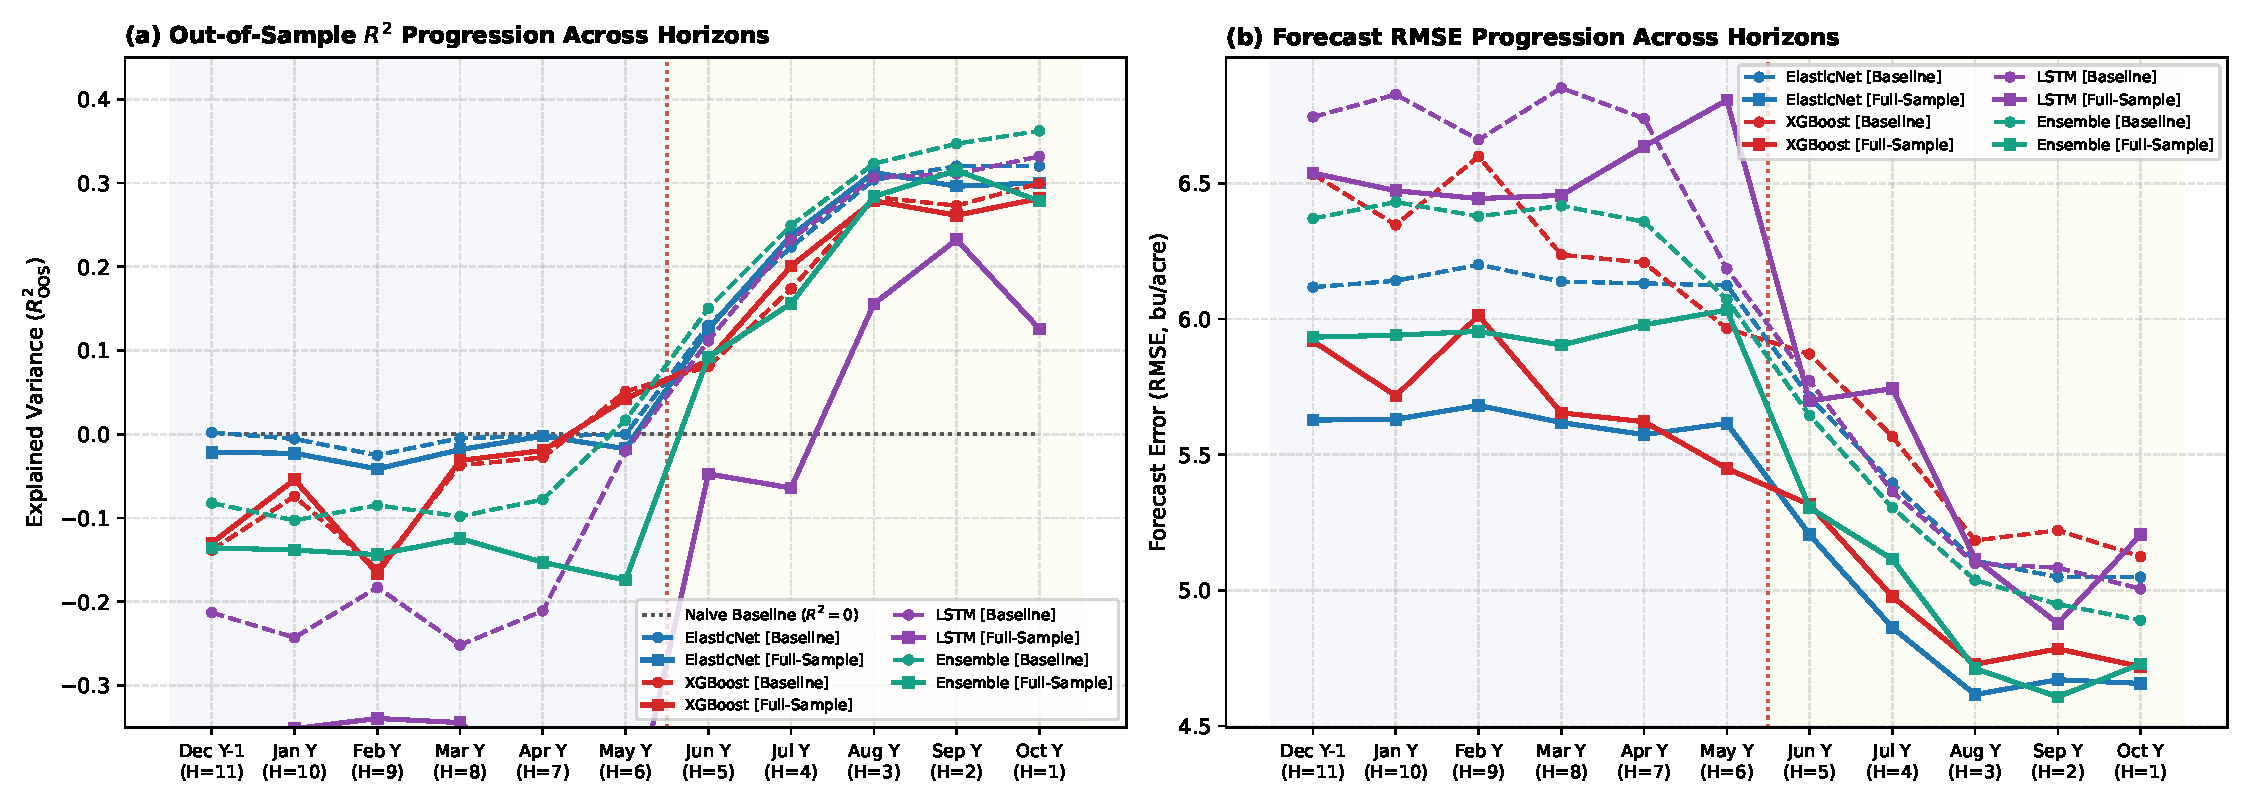
\includegraphics[width=0.82\textwidth]{figures/fig_r2_horizon_progression_comparison.pdf}
    \caption{Progressione multi-orizzonte dell'accuratezza out-of-sample ($R^2_{\text{OOS}}$ e RMSE) a confronto tra Baseline Expanding (linee tratteggiate) e Full-Sample Detrending (linee continue) per lead time decrescenti ($H = 11 \dots 1$, 2011--2025).}
    \label{fig:r2_progression_comp}
\end{figure}

\end{document}
